% Created 2020-07-27 Mon 10:44
% Intended LaTeX compiler: pdflatex
\documentclass[presentation]{beamer}
\usepackage[utf8]{inputenc}
\usepackage[T1]{fontenc}
\usepackage{graphicx}
\usepackage{grffile}
\usepackage{longtable}
\usepackage{wrapfig}
\usepackage{rotating}
\usepackage[normalem]{ulem}
\usepackage{amsmath}
\usepackage{textcomp}
\usepackage{amssymb}
\usepackage{capt-of}
\usepackage{hyperref}
\usetheme{UoB}
\author{Mark Blyth}
\date{}
\title{}
\hypersetup{
 pdfauthor={Mark Blyth},
 pdftitle={},
 pdfkeywords={},
 pdfsubject={},
 pdfcreator={Emacs 26.3 (Org mode 9.1.9)}, 
 pdflang={English}}
\begin{document}


\section{Background}
\label{sec:org49754ec}
\begin{frame}[label={sec:org44496ef}]{NODYCON}
Abstract review is back!
\end{frame}

\begin{frame}[label={sec:orgc7c01ac}]{Last week's work}
\begin{itemize}
\item Implemented Fourier discretisation
\item Compared it against splines
\item Some ideas about surrogates and CBC
\item Manuscript editing \alert{[c. 5400 words]}
\end{itemize}
\end{frame}

\section{Discretisation}
\label{sec:org2d98ff9}
\begin{frame}[label={sec:org4a0ea12}]{Discretisation}
From last time\ldots{}
\vfill
Fitting periodic splines:
\begin{enumerate}[<+->]
\item Find the period
\begin{itemize}
\item Autocorrelation or nonlinear least squares \(F_0\) estimation
\item Fourier?
\end{itemize}
\item `Stack' periods
\begin{itemize}
\item Re-label data \(t_i\)s to phase \(\phi_i = \frac{t_i}{T} \mod 1\) or \(\phi_i = t_i \mod T\)
\end{itemize}
\item Build splines model
\begin{itemize}
\item Discretisation = BSpline coefficients
\end{itemize}
\end{enumerate}
\end{frame}

\begin{frame}[label={sec:org848c8b2}]{Discretisation}
From last time\ldots{}
\vfill
Choosing knots is hard; since we're wanting a minimal knot set\ldots{}
\begin{enumerate}[<+->]
\item Choose the desired number of knots
\item Choose knots at random
\item Numerically optimize the knot vector
\begin{itemize}
\item Minimise training error of a splines model fitted with these knots
\end{itemize}
\item Repeat steps 2,3 lots, and choose the best result
\begin{itemize}
\item Helps overcome the local minima issue
\end{itemize}
\end{enumerate}
\end{frame}

\begin{frame}[label={sec:org953b5f1}]{Discretisation}
From last time\ldots{}

\begin{center}
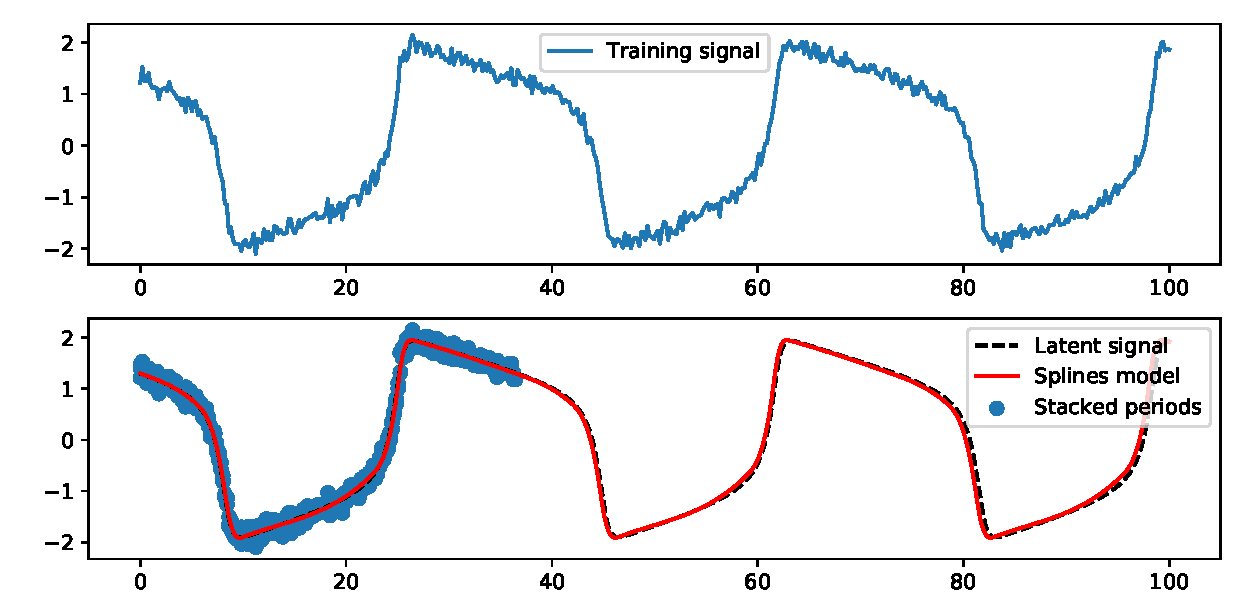
\includegraphics[width=.9\linewidth]{./fit3.pdf}
\end{center}
\end{frame}

\begin{frame}[label={sec:org29144c8}]{Discretisation}
From last time\ldots{}

\begin{center}
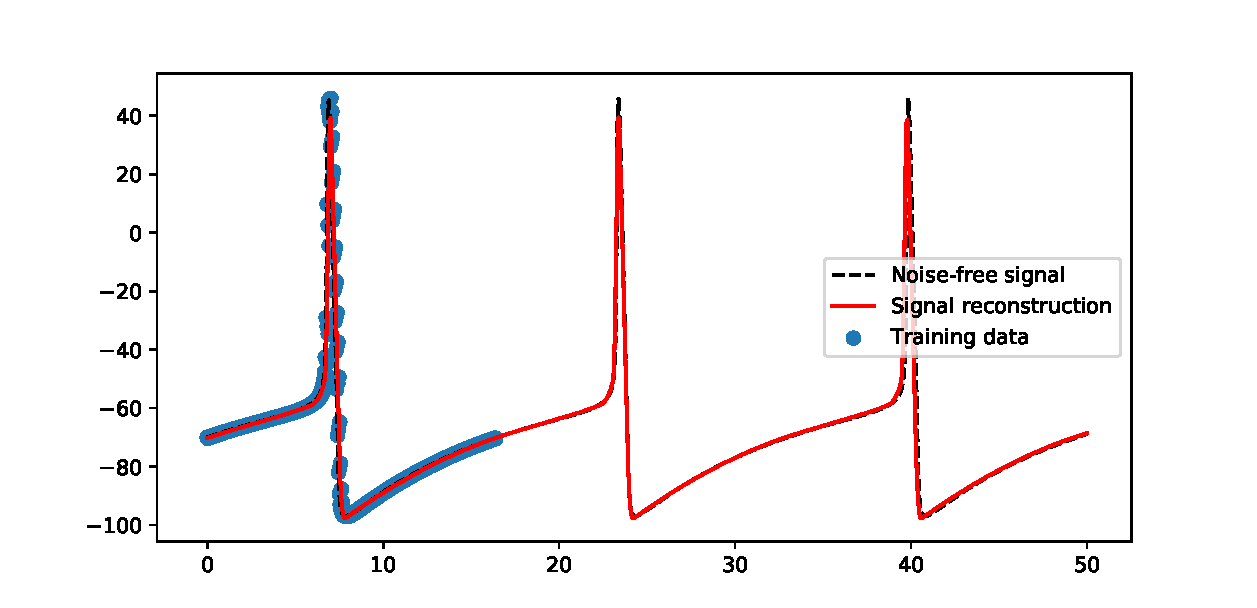
\includegraphics[width=.9\linewidth]{./HHFit2.pdf}
\end{center}
\end{frame}

\begin{frame}[<+->][label={sec:orgbf84cea}]{Discretisation}
We can quantify goodness-of-fit:
\vfill
\begin{itemize}
\item Let \(\mathrm{reconstruction}(t)\) be the fitted splines model
\item Let \(\mathrm{signal}(t)\) be the signal we wish to discretise
\item Let \(\mathrm{error}(t) = \mathrm{signal}(t) - \mathrm{reconstruction}(t)\)
\item Goodness-of-fit = \(\int_0^T\left[\mathrm{error}(t)\right]^2\mathrm{d}t\)
\item This gives a metric for comparing splines, Fourier, etc.
\end{itemize}
\end{frame}

\begin{frame}[label={sec:orga629114}]{Splines vs Fourier}
Hodgkin-Huxley neuron; error decays \emph{significantly} faster with splines
\begin{center}
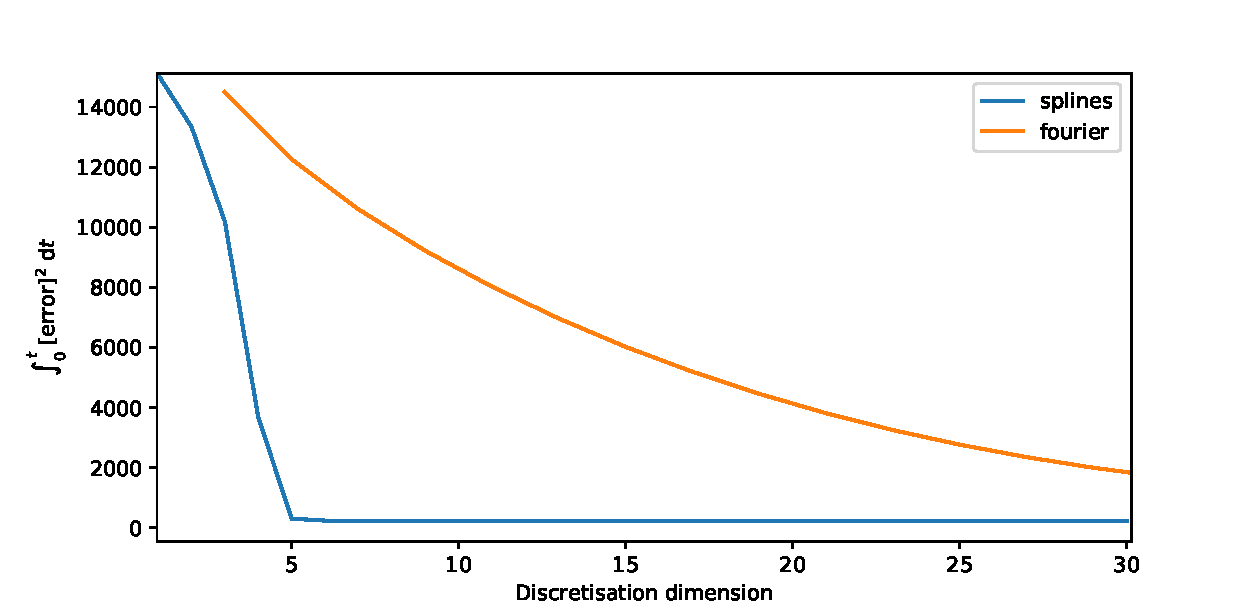
\includegraphics[width=.9\linewidth]{./HHerror2.pdf}
\end{center}
\end{frame}

\begin{frame}[label={sec:org4400509}]{Splines vs Fourier}
Hodgkin-Huxley neuron; error decays \emph{significantly} faster with splines
\begin{center}
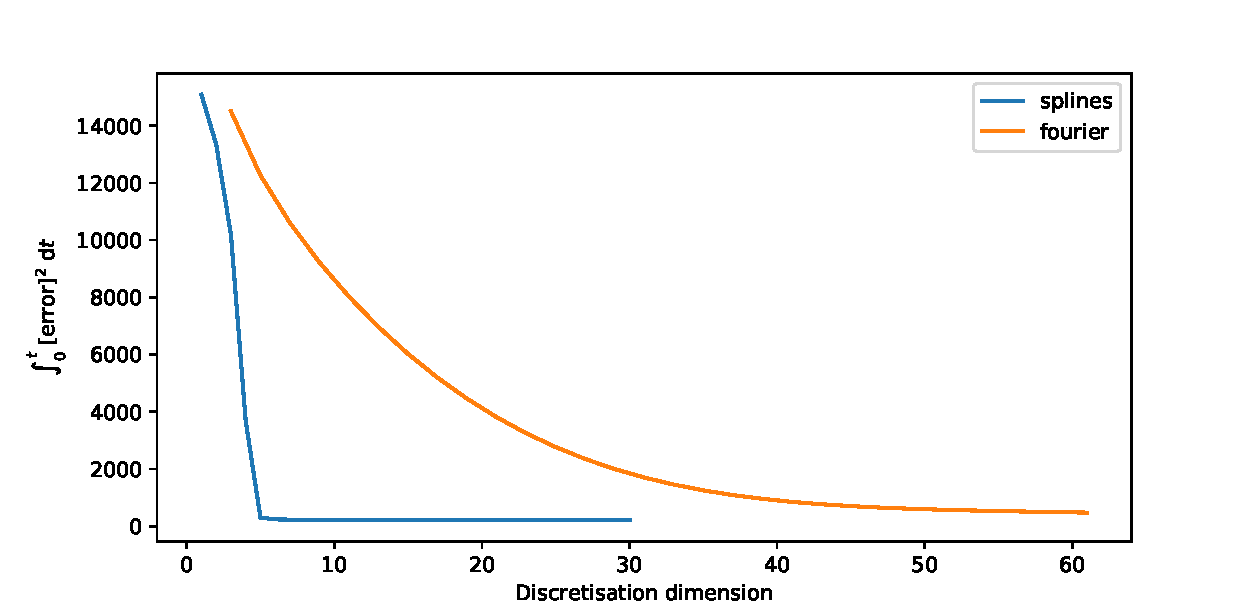
\includegraphics[width=.9\linewidth]{./HHerror.pdf}
\end{center}
\end{frame}

\begin{frame}[label={sec:org96a41ea}]{Open problems}
\begin{itemize}
\item Robustness
\begin{itemize}
\item Does it break down on stochastic systems? Eg. if data aren't fully periodic
\item Do we need a human in the loop, to manually adjust anything?
\end{itemize}
\end{itemize}
\vfill
\begin{itemize}
\item Locality
\begin{itemize}
\item Knots are fitted / work well for \(\lambda_0\); can the same knots model \(\lambda_1\), \(\lambda_2\), \dots{}, \(\lambda_i\)?
\item (They need to for predicting the next PO in an iteration)
\end{itemize}
\end{itemize}
\end{frame}

\section{CBC}
\label{sec:orgf6304a2}
\begin{frame}[label={sec:org281ac50}]{CBC approach}
Question: there's several ways of performing CBC; which is best for this?
\end{frame}

\begin{frame}[<+->][label={sec:org138bb97}]{Methods for PO CBC}
Method 1. `Easy' approach for harmonically forced systems
\vfill
\begin{itemize}
\item Set the response amplitude
\item Find the input forcing amplitude that gives that response
\item Lumps the bifurcation parameter together with the control action
\begin{itemize}
\item Fast and efficient iteration scheme
\item Similar approach exists for continuing equilibria
\end{itemize}
\end{itemize}
\end{frame}

\begin{frame}[label={sec:org04ebd72}]{Method 1 issues}
\begin{center}
We don't have a harmonically forced system
\end{center}
\end{frame}

\begin{frame}[<+->][label={sec:org607e53f}]{Methods for PO CBC}
Method 2. Harder, fully general approach \emph{[Sieber Krauskopf]}
\vfill
\begin{itemize}
\item Define the `IO map' from control-target to system output
\begin{itemize}
\item Says what the system output is, for any given control target
\end{itemize}
\item Map fixed point means control-target = system output
\item \emph{[Claim:]} map fixed point occurs only when there's non-invasive control
\item Use Newton iterations to solve for fixed point of discretised map
\item Solution is the noninvasive control target
\end{itemize}
\end{frame}

\begin{frame}[<+->][label={sec:orgf7c1125}]{Method 2 issues}
I think this is wrong\ldots{}
\begin{itemize}
\item Integral control \(\implies\) no proportional error
\item No proportional error \(\implies\) system output == control target
\begin{itemize}
\item System output exactly tracks control target
\end{itemize}
\item System output == control target \(\implies\) every control target is a fixed point of the IO map
\begin{itemize}
\item Control target and system output are identical for all targets
\end{itemize}
\item Every point is a fixed point \(\implies\) can't find noninvasive control by solving the map
\item My claim: IO-map fixed point is a necessary but not sufficient condition for noninvasiveness
\item Feels like a big claim to say the paper's wrong, but I haven't found any way to resolve this\ldots{}
\end{itemize}
\end{frame}

\begin{frame}[<+->][label={sec:org217e6fe}]{Method 2 solutions}
Approach 1. Only use P, PD control
\begin{itemize}
\item No integral controller \(\implies\exists\) proportional error
\item Proportional error = 0 \(\iff\) control action is zero (noninvasiveness)
\begin{itemize}
\item System output = control target \(\iff\) control is noninvasive
\item IO map fixed point \(\iff\) control is noninvasive
\end{itemize}
\item Can then use Newton iterations to solve for noninvasiveness
\begin{itemize}
\item Let \(\mathbf{u}^*=\) control target discretisation
\item Let \(\mathbf{x}=\) system output discretisation
\item Equality \(\implies\) no proportional error \(\implies\) zero control action, noninvasiveness, etc.
\item \(\mathbf{u}^*\) = \(\mathbf{x}\) can therefore be solved for noninvasive \(\mathbf{u}^*\)
\end{itemize}
\item This is exactly the method proposed in Sieber Krauskopf
\item Downside: locked into a single control method
\end{itemize}
\end{frame}

\begin{frame}[<+->][label={sec:orgc7878d1}]{Method 2 solutions}
Approach 2. Reformulate the zero problem
\vfill
\begin{itemize}
\item Explicitly solve for noninvasive control
\item Total control action = \(\int u(\mathbf{u^*}, t)^2\mathrm{d}t\)
\item Solve for \(\mathbf{u}^*\) that sets total control action to zero
\begin{itemize}
\item Underdetermined -- \(n\) inputs, one output; minimisation problem
\item Eg. gradient descent on \(\mathbf{u}^*\) with Broyden Jacobian update
\item This is similar to standard Newton iterations
\end{itemize}
\item Downsides: minimisation might be slower; no literature precedent
\end{itemize}
\end{frame}

\begin{frame}[label={sec:orgdf4899d}]{Optimal design of gradient-descent method}
Maybe we don't need to find \(\mathbf{u}^*\) that sets control action to zero\ldots{}
\end{frame}

\begin{frame}[<+->][label={sec:org14652ca}]{Optimal design of gradient-descent method}
\begin{itemize}
\item Much like tracking bifurcations optimally -- don't need to see the actual bifurcation point, as long as we're confident it's there
\item Find a local surrogate model of total invasiveness \(I(\mathbf{u}^*) = \int u(\mathbf{u}^*,t)^2 \mathrm{d}t\) 
\begin{itemize}
\item Maps a discretisation \(\mathbf{u}^*\) to total control action required to stabilise it
\item Quantifies invasiveness of target \(\mathbf{u}^*\)
\item \(I(\mathbf{u}^*)=0\) \(\implies\) \(u^*\) is noninvasive, so natural system behaviour
\end{itemize}
\item Solve for \(I(\mathrm{u}^*)=0\) on the local surrogate model
\begin{itemize}
\item Moves calculations out of experiment and onto computer, where they can be performed much faster
\item No need for experimental Newton iterations, gradient descent, Jacobians, finite differences
\end{itemize}
\item Fit local model on `maximally informative' datapoints
\begin{itemize}
\item Choose datapoints that maximise our certainty of the minima location
\end{itemize}
\item Experimentally test \(\mathbf{u}^*_i\) that solves \(I(\mathbf{u}^*)=0\), to ensure that's the noninvasive solution
\end{itemize}
\end{frame}

\begin{frame}[label={sec:org7b5feb6}]{Proposed route}
Initially, use PD control, IO map with Newton iterations
\begin{itemize}
\item Standard method, so don't have to develop anything new
\item Need to use PD control, but that also means no need to develop any fancy controller
\item Gets results quickly!
\end{itemize}
\vfill
\emph{If PD doesn't work well}, develop the surrogate gradient descent method
\begin{itemize}
\item Makes it truly control-strategy independent
\item Extends fully-general CBC to systems that are harder to control with PD
\end{itemize}
\end{frame}

\section{Control-free continuation}
\label{sec:org94a0829}
\begin{frame}[label={sec:org4b74bc0}]{An  aside}
Interesting aside: control-free continuation
\vfill
\begin{itemize}
\item Some systems are hard to control
\item Can we run CBC \emph{without needing a controller}?
\end{itemize}
\end{frame}

\begin{frame}[label={sec:orgdbfe774}]{Control-free continuation}
We can deduce the existence of an unstable equilibrium

\begin{center}
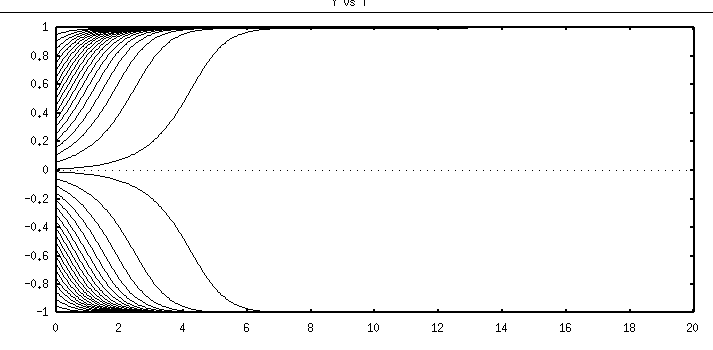
\includegraphics[width=.9\linewidth]{./bistable.png}
\end{center}
\end{frame}

\begin{frame}[<+->][label={sec:org965e5ef}]{Control-free continuation}
\begin{itemize}
\item Stable features are easy to spot -- the system converges to them
\item We can often deduce the existence of unstable features
\item Easy method: fit a local surrogate, find unstable features from that
\begin{itemize}
\item Eg. fit a neural ODE / neural GP to the previous bistable system
\item Simple root-finding for locating equilibria
\item More optimal-experimental-design opportunities, for increasing confidence at equilibrium locations
\end{itemize}
\end{itemize}
\end{frame}

\begin{frame}[<+->][label={sec:orgceef2dc}]{Control-free continuation}
General method:
\begin{enumerate}
\item Collect some data
\begin{itemize}
\item Set the system running
\item Every time instabilities drive it away from the region of interest, restart with the system where we want it
\end{itemize}
\item Reconstruct state space from recorded time series
\item Fit a neural / GP ODE model to reconstructed state space
\item Run standard analyses on the models
\begin{itemize}
\item If we keep the system near some feature of interest, the models will be locally accurate there
\item Can use standard methods to locate unstable POs from the models
\item Could use standard continuation on the models, or\ldots{}
\item \ldots{}Could find POs, UPOs at lots of parameter values, to track them without control or continuation
\end{itemize}
\end{enumerate}
\begin{itemize}
\item Nice example of what surrogates could do
\end{itemize}
\end{frame}

\begin{frame}[label={sec:org85eb5d4}]{}
\begin{center}
Back on topic\ldots{}
\end{center}
\end{frame}

\section{Surrogates}
\label{sec:org598591e}
\begin{frame}[label={sec:orgeb855be}]{When are surrogates useful?}
\begin{itemize}
\item Conference abstract discusses surrogates
\item Paper needs to make their usage cases clear
\end{itemize}
\end{frame}

\begin{frame}[label={sec:org25bf1de}]{When are surrogates useful?}
Slow signals:

\vfill
\begin{itemize}
\item No high harmonics \(\implies\) Fourier discretisation works fine \(\implies\) no need for a novel discretisation
\item No high harmonics \(\implies\) low-pass filtering works fine \(\implies\) no need for a surrogate
\end{itemize}

\vfill
No need for surrogates
\end{frame}
\begin{frame}[label={sec:org303d9eb}]{When are surrogates useful?}
Fast signals:
\vfill
\begin{itemize}
\item Lots of high harmonics \(\implies\) Fourier discretisation doesn't work \(\implies\) need a novel discretisation
\item Novel discretisation \(\implies\) no need for a surrogate as well
\end{itemize}

\vfill
No need for surrogates
\end{frame}

\begin{frame}[label={sec:orge41b66c}]{When are surrogates useful?}
Medium-speed signals:
\vfill
\begin{itemize}
\item Can be more efficiently discretised with splines than Fourier
\item Harmonically forced systems: faster to use Fourier iterations than Newton
\begin{itemize}
\item Splines discretise more efficiently, but we still use Fourier
\end{itemize}
\item Enough HF harmonics that we wouldn't want to use LP filtering \(\implies\) we need a surrogate
\end{itemize}

\vfill
This is surrogates usage case
\end{frame}

\begin{frame}[label={sec:org8336478}]{When are surrogates useful?}
\begin{itemize}
\item Better to use Fourier iterations than Newton iterations on harmonically forced systems
\item Surrogates are useful for Fourier iteration on faster signals
\item Example usage: cleaning noise from a highly nonlinear forced Duffing
\end{itemize}
\end{frame}

\begin{frame}[label={sec:orgdded98d}]{When are surrogates useful?}
\begin{center}
\begin{tabular}{lll}
Type & Harmonically forced & Unforced\\
\hline
Slow signal & Fourier iter's, LP filters & Newton iter's, LP filters\\
Fast signal & \alert{Fourier iter's, surrogates} & \uline{Newton iter's, novel discretisation}\\
\end{tabular}
\end{center}

\vfill
The two new methods complement each other; one for Newton iter's, one for Fourier iter's; paper should make this clear
\end{frame}

\section{Next steps}
\label{sec:orgcedb432}
\begin{frame}[<+->][label={sec:orgd56c5c2}]{Summary}
\begin{itemize}
\item CBC implementation should use Newton iterations, spline discretisation, PD control
\item Conference paper needs to be clear / explicit about when surrogates, new discretisations are useful
\item Interesting aside 1: we need a different approach to use non-PD control with the most general CBC method
\begin{itemize}
\item Less general methods (where parameter and control action can be lumped together) don't require this
\item Lots of room for interesting optimal experimental design
\end{itemize}
\item Interesting aside 2: might be possible to run CBC without a controller?
\end{itemize}
\end{frame}

\begin{frame}[label={sec:org85e20cf}]{Next steps}
\begin{enumerate}
\item Test splines generalisation, robustness
\item Write up results so far into a paper
\item Demonstrate splines with CBC
\end{enumerate}

\vfill
Alternative: skip step 1 altogether and jump in with CBC simulation
\end{frame}

\begin{frame}[label={sec:org1e950a4}]{Generalisation and robustness [again]}
\begin{itemize}
\item Generalisation
\begin{itemize}
\item Knots are fitted / work well for \(\lambda_0\); can the same knots model \(\lambda_1\), \(\lambda_2\), \dots{}, \(\lambda_i\)?
\item (They need to for predicting the next PO in an iteration)
\end{itemize}
\end{itemize}
\vfill
\begin{itemize}
\item Robustness
\begin{itemize}
\item Does it break down on stochastic systems? Eg. if data aren't fully periodic
\item Do we need a human in the loop, to manually adjust anything?
\end{itemize}
\end{itemize}
\end{frame}

\begin{frame}[label={sec:org72cde9b}]{Key dates}
\begin{itemize}
\item Bath maths ML conference, week of Aug.3rd - 7th
\item Conference paper submission, September \sout{11th} 25th
\item Goal: start conference paper writing mid-August
\end{itemize}
\end{frame}
\end{document}
